\documentclass[finnish,english]{beamer}
%\documentclass[finnish,english,handout]{beamer}

% Uncomment if want to show notes
%\setbeameroption{show notes}

\mode<presentation>
{
  \usetheme{Warsaw}
  % oder ...

  %\setbeamercovered{transparent}
  % oder auch nicht
}


%\usepackage[pdftex]{graphicx}
\usepackage[T1]{fontenc}
\usepackage[latin1]{inputenc}
%\usepackage[T1,mtbold,lucidacal,mtplusscr,subscriptcorrection]{mathtime}
\usepackage{times}
\usepackage{epic,epsfig}
\usepackage{subfigure,float}
\usepackage{amsmath,amsfonts,amssymb}
\usepackage{inputenc}
\usepackage{babel}
%\usepackage{euscript}
\usepackage{afterpage}
%\usepackage{picinpar}
%\usepackage{array,longtable}
\usepackage{url}
\urlstyle{same}
\usepackage{eufrak}
\usepackage{amsbsy}
\usepackage{eucal}
\usepackage{rotating}

\usepackage{natbib}
\bibliographystyle{apalike}

% \definecolor{hutblue}{rgb}{0,0.2549,0.6784}
% \definecolor{midnightblue}{rgb}{0.0977,0.0977,0.4375}
% \definecolor{navyblue}{rgb}{0,0,0.5}
% \definecolor{hutsilver}{rgb}{0.4863,0.4784,0.4784}
% \definecolor{lightgray}{rgb}{0.95,0.95,0.95}
% \definecolor{section}{rgb}{0,0.2549,0.6784}
% \definecolor{list1}{rgb}{0,0.2549,0.6784}
% \renewcommand{\emph}[1]{\textcolor{navyblue}{#1}}

\graphicspath{../luku1}

\pdfinfo{
          /Title      (Bayesian data analysis)
          /Author     (Aki Vehtari) %
          /Keywords   (Bayesian probability theory, Bayesian inference, Bayesian data analysis)
}


\parindent=0pt
\parskip=8pt
\tolerance=9000
\abovedisplayshortskip=0pt

\setbeamertemplate{navigation symbols}{}
\setbeamertemplate{headline}[default]{}
\setbeamertemplate{headline}[text line]{\insertsection}
\setbeamertemplate{footline}[frame number]


\def\o{{\mathbf o}}
\def\t{{\mathbf \theta}}
\def\w{{\mathbf w}}
\def\x{{\mathbf x}}
\def\y{{\mathbf y}}
\def\z{{\mathbf z}}

\DeclareMathOperator{\E}{E}
\DeclareMathOperator{\Var}{Var}
\DeclareMathOperator{\var}{var}
\DeclareMathOperator{\Sd}{Sd}
\DeclareMathOperator{\sd}{sd}
\DeclareMathOperator{\Bin}{Bin}
\DeclareMathOperator{\Beta}{Beta}
\DeclareMathOperator{\logit}{logit}
\DeclareMathOperator{\N}{N}
\DeclareMathOperator{\U}{U}
\DeclareMathOperator{\BF}{BF}
%\DeclareMathOperator{\Pr}{Pr}
\def\euro{{\footnotesize \EUR\, }}
\DeclareMathOperator{\rep}{\mathrm{rep}}


\title[]{Bayesian data analysis}
\subtitle{Practical matters}

\author{Aki Vehtari}

\institute[Aalto University]{}

\begin{document}

\section{Course contents}


\begin{frame}
  \frametitle{Bayesian data analysis (Aalto fall 2018)}  %
  \framesubtitle{}
  \begin{itemize}
  \item Book: Gelman, Carlin, Stern, Dunson, Vehtari \& Rubin: Bayesian Data
    Analysis, Third Edition.
  \item Timetable: Lectures on Mondays at 14-16, TAs available Thursdays 12-16, Fridays 10-12
    \begin{itemize}
    \item TAs: Michael Riis Andersen, Akash Dhaka, M�ns Magnusson,
      Topi Paananen, Juho Piironen, Eero Siivola, Tuomas Sivula
    \end{itemize}
  \end{itemize}
 \begin{center}
   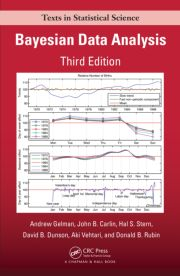
\includegraphics[width=3cm]{figs/BDA3.jpg}
 \end{center}

\end{frame}

\begin{frame}
  \frametitle{Bayesian data analysis}  %
  \framesubtitle{Pre-requisites}
  \begin{itemize}
  \item Basic terms of probability theory
    \begin{itemize}
    \item probability, probability density, distribution
    \item sum, product rule, and Bayes' rule
    \item expectation, mean, variance, median
    \end{itemize}
  \item Some algebra and calculus
  \item Basic visualisation techniques (R or Python)
    \begin{itemize}
    \item histogram, density plot, scatter plot
    \end{itemize}
  \end{itemize}

  These will be tested with the first assignment round

\end{frame}

\begin{frame}
  \frametitle{Bayesian data analysis}  %
  \framesubtitle{Course contents}
  \begin{itemize}
  \item Background (Ch 1)
  \item Single-parameter models (Ch 2)
  \item Multiparameter models (Ch 3)
  \item Computational methods (Ch 10)
  \item Markov chain Monte Carlo (Ch 11--12)
  \item Stan and probabilistic programming
  \item Hierarchical models (Ch 5)
  \item Model checking (Ch 6)
  \item Evaluating and comparing models (Ch 7)
  \item Decision analysis (Ch 9)
  \item Large sample properties and Laplace approximation (Ch 4)
  \item In addition you learn workflow for Bayesian data analysis
  \end{itemize}
  
\end{frame}

\begin{frame}
  \frametitle{Bayesian data analysis}  %

  \begin{itemize}
  \item Lectures describe basics and give broader overview
    \begin{itemize}
    \item part of lecture time for questions
     \item written material has all the details and self-study
       is possible
    \end{itemize}
  \item Supporting material, assignments and news in MyCourses
  \item Supporting material and assignments in \url{https://github.com/avehtari/BDA_course_Aalto}
    \begin{itemize}
    \item reading instructions and chapter notes
    \item demos
    \item slides
    \item links to additional material
    \end{itemize}
  \item R demos \url{https://github.com/avehtari/BDA_R_demos/}
  \item Python demos \url{https://github.com/avehtari/BDA_py_demos/}
  \item Slack channel
  \end{itemize}

\end{frame}

\begin{frame}
  \frametitle{Bayesian data analysis}  %
  \framesubtitle{Exercises}
  \begin{itemize}
  \item Exercises are given on PeerGrade (also available in git repo)
  \item Exercises are returend and graded on Peergrade
  \item R/Python simulation exercises
  \item Stan exercises (via R/Python)
    \begin{itemize}
    \item Stan is a probabilistic programming language implementing
      full Bayesian statistical inference
    \end{itemize}
  \end{itemize}
\end{frame}

\begin{frame}
  \frametitle{Bayesian data analysis}  %
  \framesubtitle{Computer exercises}
  \begin{itemize}
  \item Basic visualisation techniques
  \item Binomial distribution -- Algae
  \item Normal distribution -- Windshield
  \item Difference between binomials -- Treatment/control
  \item Difference between normals -- Windshield
  \item Generalized linear model (GLM) + importance sampling -- Bioassay
  \item GLM + Metropolis + convergence diagnostics -- Bioassay
  \item GLM + Bioassay + Stan
  \item Linear model + Stan
  \item Hierarchical model + Stan
  \item Model seletion + Stan
  \end{itemize}

\end{frame}

\begin{frame}
  \frametitle{Bayesian data analysis}  %
  \framesubtitle{Example analyses}
  \begin{itemize}
  \item Treatment/control
    \begin{itemize}
    \item randomize patients to treatment or control
    \item is the treatment effective?
    \end{itemize}
    \pause
  \item Continuous valued treatment
    \begin{itemize}
    \item randomize patients with different dosages
    \item which dosage is sufficient without too many side effects?
    \end{itemize}
    \pause
  \item Different effects for different patients?
    \begin{itemize}
    \item Is the treatment effect different for male/female, child/adult, light/heavy, ...
    \end{itemize}
  \end{itemize}

\end{frame}

\begin{frame}
  \frametitle{Bayesian data analysis}  %
  \framesubtitle{Assessment}
  \begin{itemize}
  \item Exercises (48p) and project work (24p\%)
     \begin{itemize}
     \item Minimum of 50\% of points must be obtained from both the exam and the exercises.
     \item Preliminary grade boundaries\\
       <50\%=0, 50\%-60\%=1, 60\%-70\%=2, 70\%-80\%=3, 80\%-90\%=4, >90\%=5
     \end{itemize}
  \end{itemize}

\end{frame}

\begin{frame}
  \frametitle{Bayesian data analysis}  %
  \framesubtitle{Exercises}
  \begin{itemize}
  \item Weekly exercises introduced on Monday lecture
  \item Related R/Python demos available
  \item TAs available on Thursday 12--16 and Friday 10--12
  \item Exercise deadlines on Sunday (see detailed info in MyCourses)
  \item After exercise deadline grading period Monday--Tuesday
  \item Students grade 4 other exercises using peergrade.io
  \end{itemize}

\end{frame}

\begin{frame}
  \frametitle{Exercises}  %
  \framesubtitle{peergrade.io}
  \begin{itemize}
  \item Used in BDA course since 2016
  \item Each student grades 4 exercises (randomly distributed)
  \item Detailed grading instructions
  \item Also text feedback
  \item Possible to flag inappropriate grading
  \item TAs check flagged gradings and strongly coflicting gradings
  \item Possible to give thumb up for great feedback
    \begin{itemize}
    \item those who give good feedback will get bonus points
    \end{itemize}
  \end{itemize}
  
\end{frame}

\begin{frame}
  \frametitle{Exercises}  %
  \framesubtitle{peergrade.io}

  \begin{itemize}
  \item Combined score: 70\% submission performance, 30\% feedback performance
    \pause
  \item Hand-in score:
    \begin{itemize}
    \item averaging the scores from peers
    \item after flagging teacher may overrule the score
    \item different exercises have different weight
    \end{itemize}
    See details at \url{http://help.peergrade.io/interfaces-and-features/grading-and-scores/the-hand-in-score}
    \pause
  \item Feedback score:
    \begin{itemize}
    \item The constructive score
    \item The hand-in evaluation accuracy score
    \item The feedback evaluation accuracy score
    \item The feedback completeness score
    \item The feedback evaluation completeness score
    \end{itemize}
    See details at \url{http://help.peergrade.io/interfaces-and-features/grading-and-scores/the-feedback-score}
  \end{itemize}
  
\end{frame}

\begin{frame}
  \frametitle{Project work}  %
  \framesubtitle{}
  \begin{itemize}
  \item Project work in groups of 2--3
    \begin{itemize}
    \item combines all the pieces in one project work
    \item R or Python notebook report
    \item project report peer graded
    \item oral presentation 
    \end{itemize}
  \end{itemize}
  
\end{frame}


\end{document}

%%% Local Variables:
%%% mode: latex
%%% TeX-master: t
%%% End:
